
\documentclass{beamer}

\mode<presentation>
{
\usetheme{Warsaw}

\setbeamercovered{transparent}
}

\usepackage[english]{babel}
\usepackage[latin1]{inputenc}

% font definitions, try \usepackage{ae} instead of the following
% three lines if you don't like this look
\usepackage{mathptmx}
\usepackage[scaled=.90]{helvet}
\usepackage{courier}


\usepackage[T1]{fontenc}


\title{Gestion de Projets}

%\subtitle{}

% - Use the \inst{?} command only if the authors have different
%   affiliation.
%\author{F.~Author\inst{1} \and S.~Another\inst{2}}
\author{Anthony CAILLAUD Charles DEJEAN Mano�l FORTUN}

% - Use the \inst command only if there are several affiliations.
% - Keep it simple, no one is interested in your street address.
%\institute[Universities of]
% {
% \inst{1}%
% Department of Computer Science\\
% Univ of S
% \and
% \inst{2}%
% Department of Theoretical Philosophy\\
% Univ of E}

\date{10/02/2011}


% This is only inserted into the PDF information catalog. Can be left
% out.
\subject{Talks}



% If you have a file called "university-logo-filename.xxx", where xxx
% is a graphic format that can be processed by latex or pdflatex,
% resp., then you can add a logo as follows:

% \pgfdeclareimage[height=0.5cm]{university-logo}{university-logo-filename}
% \logo{\pgfuseimage{university-logo}}



% Delete this, if you do not want the table of contents to pop up at
% the beginning of each subsection:
\AtBeginSection[]
{
\begin{frame}<beamer>
\frametitle{Outline}
\tableofcontents[currentsection,hideothersubsections]
\end{frame}
}



\begin{document}

\begin{frame}
\titlepage
\end{frame}



\begin{frame}
\frametitle{Table of Contents}
\tableofcontents[hideallsubsections]
\end{frame}

\section{Notre Entreprise}

\begin{frame}\frametitle{Pr�sentation de notre entreprise}

\begin{itemize}
\item BamZiGitty créée en 2011
\item Java, pas C++ même sous la torture
\item Monde libre
\end{itemize}


\end{frame}

\section{Notre équipe}
\begin{frame}\frametitle{Une équipe}

\begin{itemize}
\item Bambinome
\item Gros tony
\item Zigmon
\item Hello Gitty
\item John Bob ingénieur 5 ans expérience
\item Bob technicien tout neuf
\item Arnaud fantome
\end{itemize}


\end{frame}


\section{Planning et Plan de Charge}

\begin{frame}\frametitle{Planning et Plan de Charges}
\begin{figure}[t]
  		\centering
  		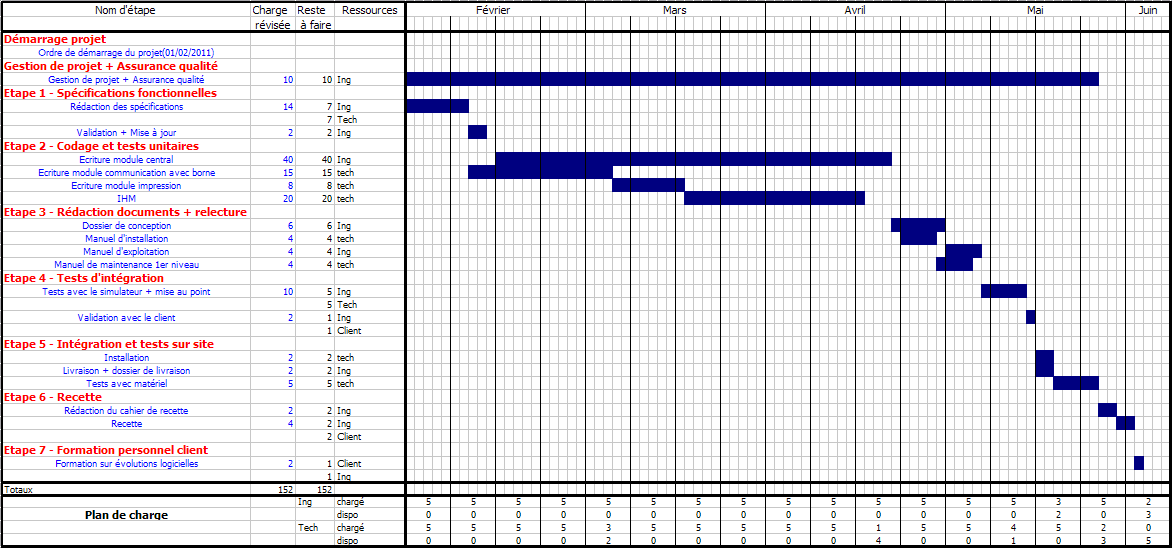
\includegraphics[height=6cm,width=11cm]{images/Planning.PNG}
  		\caption{Planning et Plan de Charges}
  		\label{Planning}
	\end{figure}
\end{frame}

\section{Journal d'actions}

\begin{frame}\frametitle{Journal d'actions}
\begin{figure}[t]
  		\centering
  		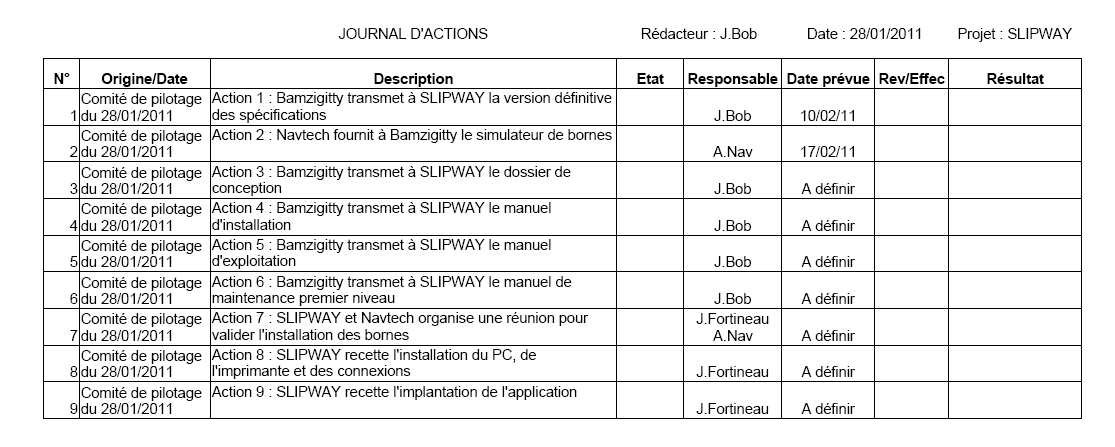
\includegraphics[height=5cm,width=11cm]{images/journal_dactions.PNG}
  		\caption{Journal d'actions}
  		\label{JournalActions}
	\end{figure}
\end{frame}



section{Prix de vente}

\begin{frame}\frametitle{Prix de vente}

$ prix vente= Prix revient employé + prix vente matériel $ 
$ prix vente mat= \frac {prix achat} {1-marge} $
$ prix revient employ� = \frac {prix total employé + garantie} { 1-marge} $
$ Marge = 25\% $

\end{frame}
\begin{frame}

\begin{figure}[t]
\centering
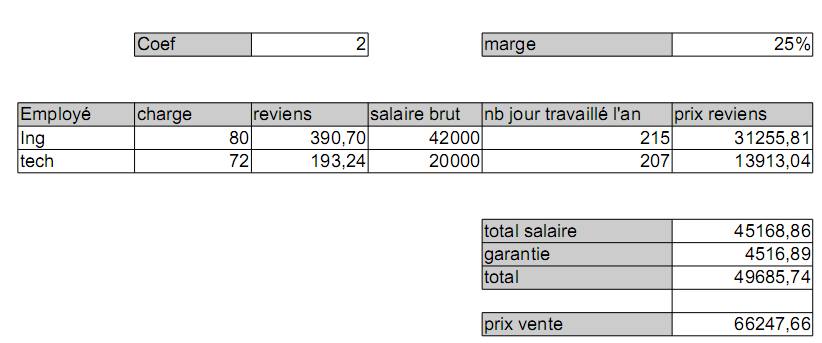
\includegraphics[height=5cm,width=11cm]{images/prix1.PNG}
\caption{prix 1}
\label{prix 1}
\end{figure}
\end{frame}
\begin{frame}



\begin{figure}[t]
\centering
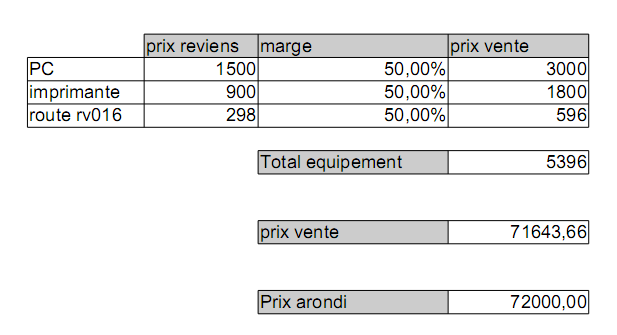
\includegraphics[height=5cm,width=11cm]{images/prix2.PNG}
\caption{prix 2}
\label{prix 2}
\end{figure}


\end{frame}

\section{Ech�ancier de facturation et conditions de paiement}
\begin{frame}\frametitle{Echéancier}

\begin{figure}[t]
\centering
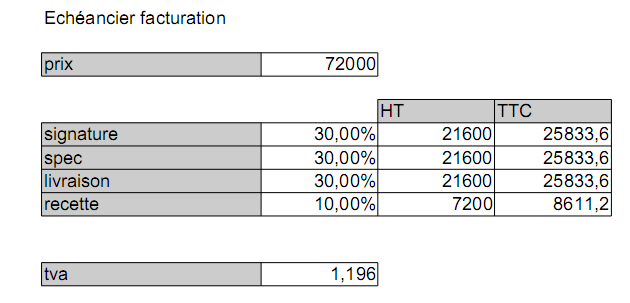
\includegraphics[height=5cm,width=11cm]{images/echancier.PNG}
\caption{echancier}
\label{echancier}
\end{figure}


\end{frame}


\begin{frame}\frametitle{Conditions de paiement}
\begin {itemize}
\item A 30 jours fin de mois le 10
\item Compte effectué le 15
\item Par virement de préférence
\end {itemize}
\end{frame}


\section{Conclusion}
\begin{frame}\frametitle{Conclusion}

\begin {itemize}
\item Assurance Périls
\item Concurents mauvais
\item Equipe à l'écoute compétente
\item Client important
\item Chaque projet compte
\item Formation et pédagogie
\item Prix
\item garantie matériel

\end {itemize}

\end{frame}


\end{document}

